\section{Application Overview}
\label{sec:app}
In the following chapter a short introduction to the actual system will be given. An entity relationship diagram explains the core data foundation of this project in \autoref{sub:db}, which includes the representation of the \gls{SKB} as described in \autoref{sub:SKB}. The general process, core functionalities and the gls{ui} will be presented in \autoref{sub:process}-\ref{sub:ui}. This is followed by a typical walkthrough to create a new analysis as a clinician. 

The application is available on \href{https://small-data-analyst.herokuapp.com}{https://small-data-analyst.herokuapp.com} and these steps can be reproduced in the demo application. At the end of this chapter a short discussion on observations is included, providing as well the insight feedback of an actual statistician using the software. A detailed view on some key components of the software can be found in \autoref{sec:implementation}.


To test the application the standard \textit{ovarian}-dataset available in \texttt{R} has been used. In addition to that, I. Sassoon provided an anonymised version of a larger clinical data set (see \autoref{app:dataset}). The description of the dataset can be found in \autoref{fig:dataset}. Possible research question arising from this dataset are presented in \autoref{fig:dataset:rq}.



\subsection{Entity Relationship Class Diagram }
\label{sub:db}


The underlying database structure of the developed application is mostly influenced by the \gls{SKB} and the representation of \texttt{Assumptions} as classes. \autoref{fig:er} shows an overview over most of the involved database models used in this application. Additional classes like \texttt{Users}, \texttt{Abilities}, etc. are intentionally left out as this would add an additional level of complexity. 

\begin{figure}[!h]
	\centering
	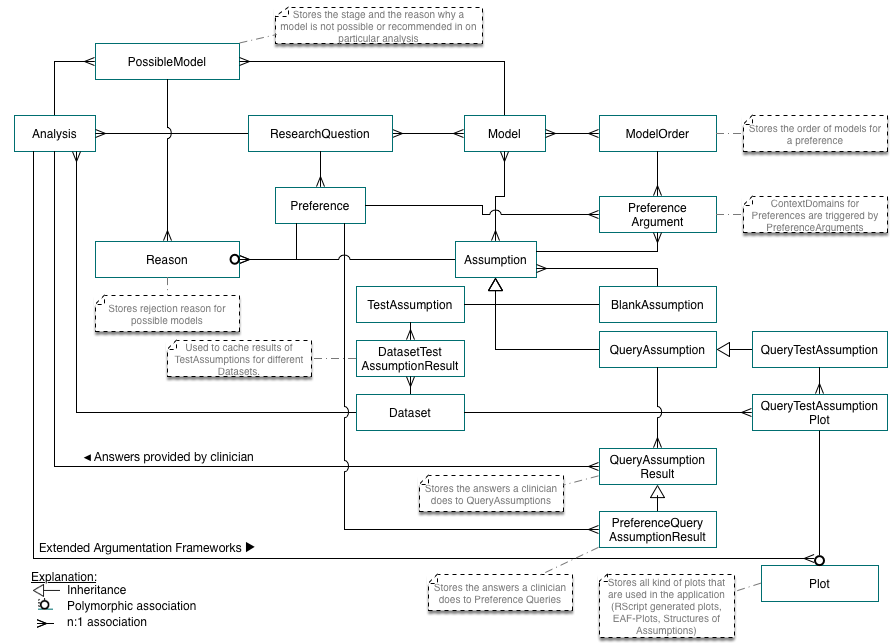
\includegraphics[width=\textwidth]{figures/er_complete}
	\caption{Entity-Relationship Diagram of the major classes used int the application. }
	\label{fig:er}
\end{figure}


The most important class is the \texttt{Analysis} which is associated with a \texttt{Dataset}, a \texttt{ResearchQuestion}, has many answered or open \texttt{QueryAssumptionResults} (this class stores the answers of a clinician to one particular \texttt{QueryAssumption}), and a list of \texttt{PossibleModels} (including impossible models and there \texttt{Reason} why they got rejected). 

The \gls{SKB} is represented by \texttt{ResearchQuestions} that have and belong to many \texttt{Models}. Each of these has multiple \texttt{Assumptions} that need to hold for this \texttt{Model}. These \texttt{Assumptions} have different specialisations: 

\bigskip

\begin{itemize}

	\item \texttt{TestAssumption}: An assumption that requires a \texttt{R} script to be executed and to return \texttt{true} or \texttt{false}. These assumptions will be checked automatically from the system and rely only on the dataset used in an analysis.
	\item \texttt{QueryAssumption}: A clinician has to provide a \textit{yes} or \textit{no} answer to a question during the process of the analysis. Only if he answers positively, this assumption holds.
	\item \texttt{QueryTestAssumption}: A \texttt{R} script generates a plot based on the dataset, which is then presented to the user who has to confirm that the plot shows some required features.
	\item \texttt{BlankAssumption}: An assumption that represents a grouping ability for other assumptions. All assigned assumptions (regardless of their type) must hold. 
\end{itemize}
\bigskip


\texttt{Preferences} have different \texttt{PreferenceArguments} that represent a specific \gls{CD} which are assigned to a particular \texttt{ModelOrder}. This allows the representation of \glspl{CD}, their order and the expressed preferences as described in \autoref{sub:SKB} in a generic way without limiting the triggers for a \gls{CD} to any particular \texttt{Assumption} type. 

The class \texttt{DatasetTestAssumptionResult} stores for each \texttt{TestAssumption} and each \texttt{Dataset} a pre-calculated result to enhance the speed of the evaluation during new \texttt{Analses}. \texttt{PreferenceQueryAssumptionResults} and \texttt{QueryAssumptionResults} store the answers of clinicians to \texttt{(Test)QueryAssumptions} for one particular \texttt{Analysis}.


\subsection{General Process and Application Setup}
\label{sub:process}
The crucial role in the process of enabling clinicians to analyse their clinical data is played by the statistician: registered or approved by an administrator they are allowed to perform significant changes to the \gls{SKB} which is required to provide the clinicians with a sophisticated foundation for their analyses. 

\begin{figure}[htbp]
\centering
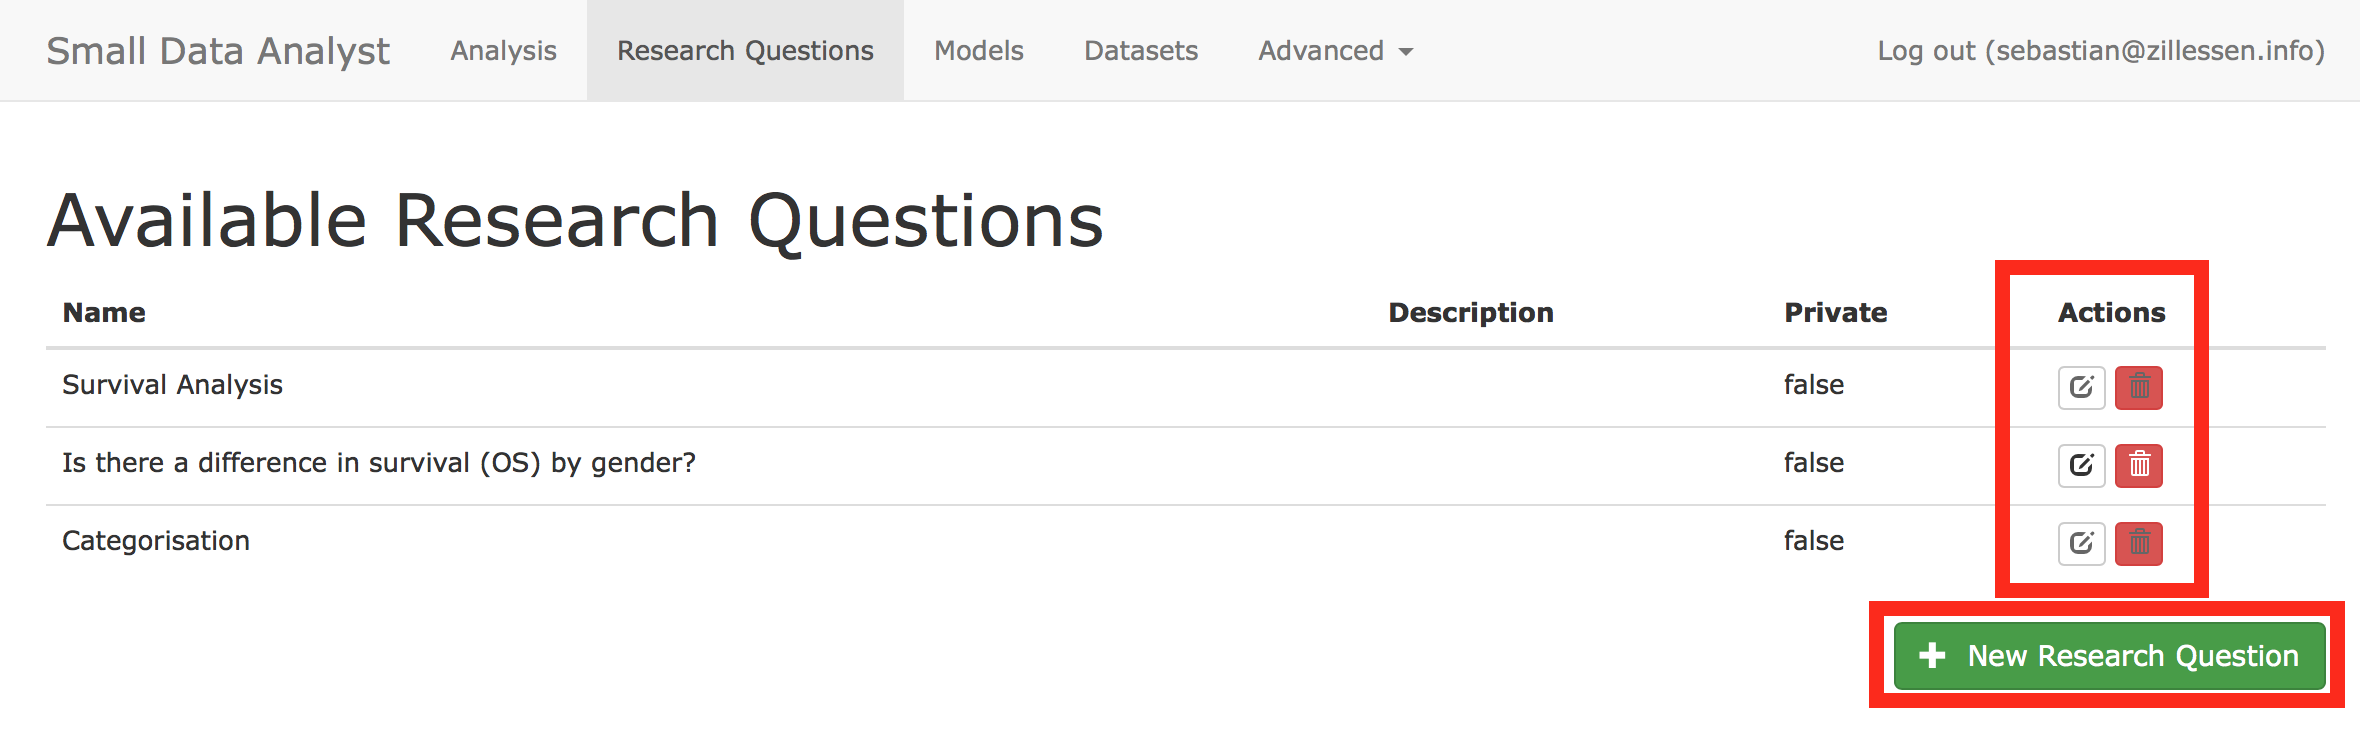
\includegraphics[width=0.8\textwidth]{figures/ui_RQ}
\caption{Listing of research questions: The highlighted areas might not be available, depending on the access rights of the currently logged-in user.}
\label{fig:ui:rq}
\end{figure}

To do so a \textbf{statistician} will first prepare the system involving the following steps:

\begin{enumerate}
	\item Defining a research question (see \autoref{fig:ui:rq}).
	\item Assigning suitable models (see \autoref{fig:ui:model}) to a research question.
	\item Providing assumptions (see \autoref{fig:ui:assumption}) that need to hold to make this model a possible model in a particular analysis.
	\item Defining (global) preferences to express a particular order between models in certain contexts that apply if a certain assumption holds (see \autoref{fig:ui:preference}).
\end{enumerate}

\bigskip

A \textbf{clinician} can then initialise a new analysis by performing the following steps:
 
\begin{enumerate}
	\item Uploading a data set that has been acquired during a clinical study.
	\item Optionally expressing (private) preferences between different models.
	\item Generating a new analysis related to a research question and providing the answers required by the system to generate a list of possible models.
	\item Answering further questions that might arise during the evaluation of the possible models to apply context domain specific preferences on the data set.
\end{enumerate}
\bigskip

By applying this workflow, \textbf{clinicians} will be able to make data-driven decisions that are based on the expertise entered by a \textbf{statistician}.


\subsection{User Interface and Core Functionalities}
\label{sub:ui}

The \gls{UI} is intentionally kept clean for simplicity reasons: \texttt{Bootstrap} is used to provide a consistent look \& feel and responsiveness of the application. As described in \autoref{sub:sassoon:actors} we have three main users in our system which have different abilities\footnote{Abilities are access rights, that are specified via an \texttt{Ability} class that is used by \texttt{cancancan} to provide diversified access-rights to different user groups in our system.} influencing the appearance of the \gls{UI} (eg. a clinician will not be able to create, alter or delete any research questions, however he will still be able to see them as depicted in \autoref{fig:ui:rq}). This approach allows us to use the same \gls{UI}-components for different users without writing them once again (\gls{DRY} principle).

\begin{figure}[h]
\centering
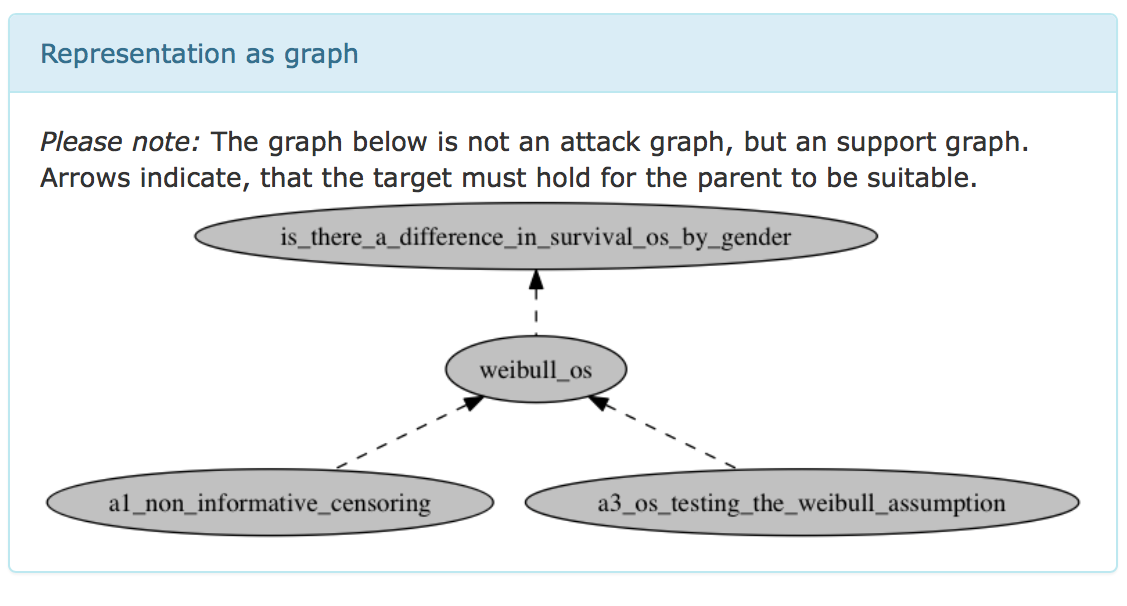
\includegraphics[width=0.8\textwidth]{figures/ui_Weibull_Model}
\caption{Overview over a model, in this particular case the \textit{Weibull model} which requires two assumptions to hold.}
\label{fig:ui:model}
\end{figure}


To provide easier access to the underlying \gls{SKB}, research questions and models include a visual representation of their relations as a graph (see lower right part of \autoref{fig:ui:model}). The system offers four different types of assumptions which have special functionalities (see \autoref{fig:ui:assumption}, explanation of each type can be found in \autoref{sub:db}).

\begin{figure}[t!]
\centering
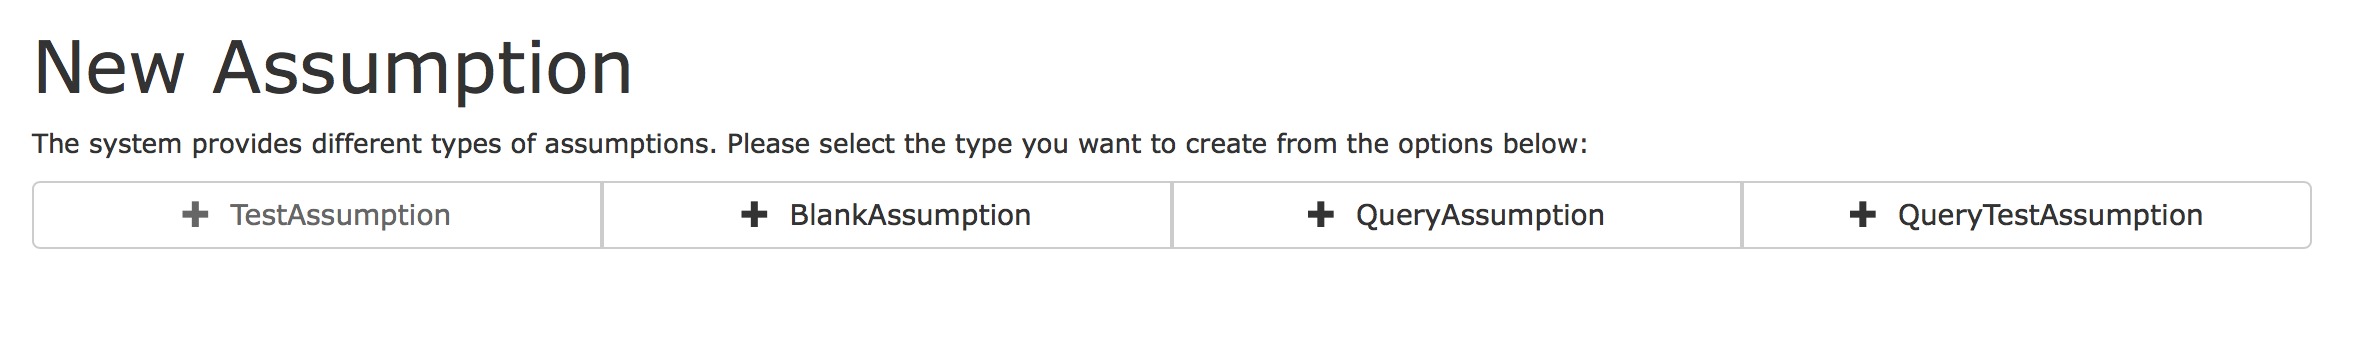
\includegraphics[width=0.8\textwidth]{figures/ui_new_assumption}
\caption{The system provides four different types of assumptions: Test, Query, Test-Query, and Blank assumptions.}
\label{fig:ui:assumption}
\end{figure}

Each of those require different attributes which results in different forms during the creation process of new assumptions. For a model to be possible during an analysis, all assumptions assigned to this model need to hold (evaluate to true) regardless of its type. In a second step, the defined \glspl{preference} are evaluated. To do so, all possible models are added to an \gls{EAF} attacking each other as described in \autoref{sub:preferences} and the \glspl{CD} are then added iteratively. This process can be seen in \autoref{fig:analysis:eaf}.

\begin{figure}[!hbt]
	\centering
	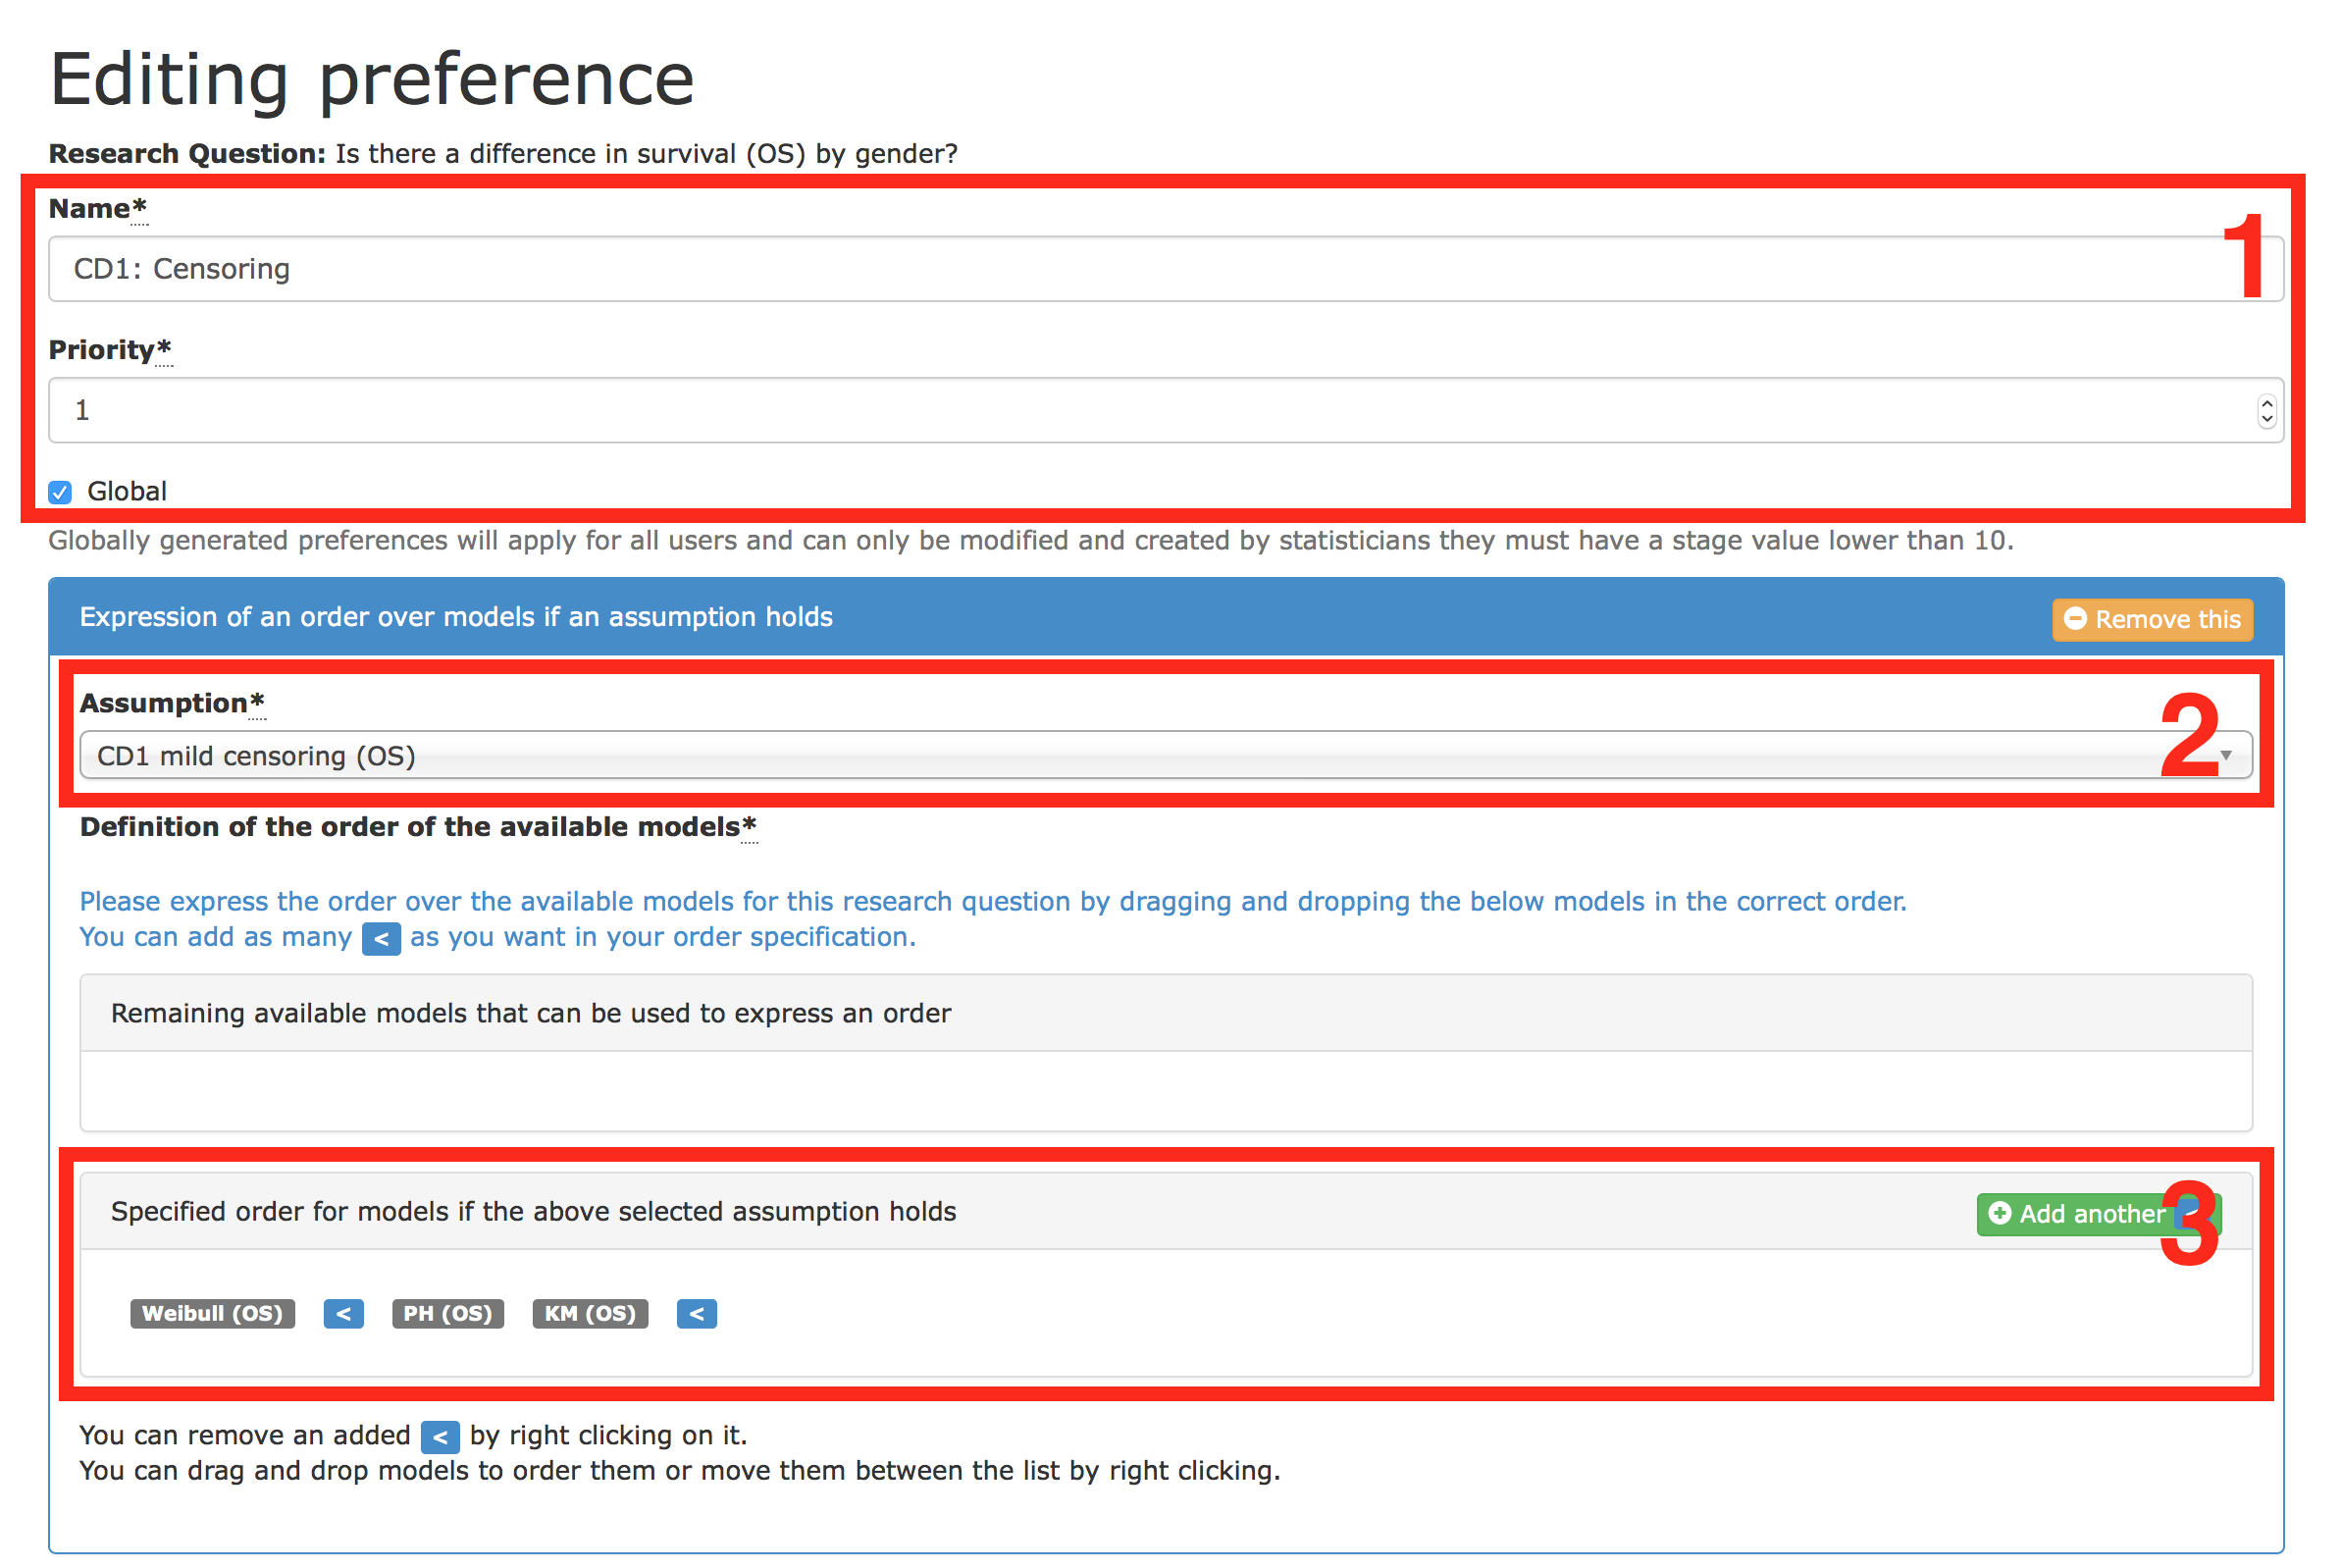
\includegraphics[width=\textwidth]{figures/ui_preference}
	\caption{\gls{UI} to enter preferences between models: General information about this preference including the applicable research question (1), the context under which this preference applies can be defined as assumption (2), and the actual order of the models can be interactively arranged per drag \& drop (3).}
	\label{fig:ui:preference}
\end{figure}


The most complex component from a \gls{UI} perspective are preferences, as they involve context domains and there required assumptions and relative orders per context domain. \autoref{fig:ui:preference} shows how this has been solved: (1) allows the user to enter general details for a preference (availability to users, rank of the preference and a name). 

For each available context domain for this particular preference, an assumption (2) has to be chosen. A context domain will be applied, if and only if this assumption holds. The relatively order between models can be specified easily via drag \& drop (3). 

This order will be taken into account when analysing the \gls{EAF} at the final step of the analysis process. If a preference is not defined over all available models for a particular research question, the model will not be attacked by any \gls{CD}, therefore the performance measurement for this model is undefined and it will stay untouched.

As expressed earlier before, the priority of a preference can be set and defines the order of applying different \glspl{CD}. This ensures, that a clinicians preference will always be less important than the statistical reasons a statistician has entered into the system ensuring reliability and statistical correctness while applying the preferences on possible models.



\subsection{Example walkthrough}
\label{sub:walk}

The following subsection describes a walkthrough for a new analysis involving a sample data set provided by I. Sassoon (see \autoref{app:dataset}) and a survival analysis by gender (preferences set according to \cite{sassoon2016CD}). These initial options are selected in \autoref{fig:analysis:1}. The following screen (see \autoref{fig:analysis:2}) shows the actual analysis screen. All \texttt{TestAssumptions} have already been evaluated and on the left hand side of the screenshot the \textit{Currently Possible Models} are depicted. On the right hand side the \textit{Open Query Assumptions} are presented to the user including one \texttt{QueryTestAssumption} with a generated plot for this particular data set and one \texttt{QueryAssumption}. 

\begin{figure}[h]
	\centering
	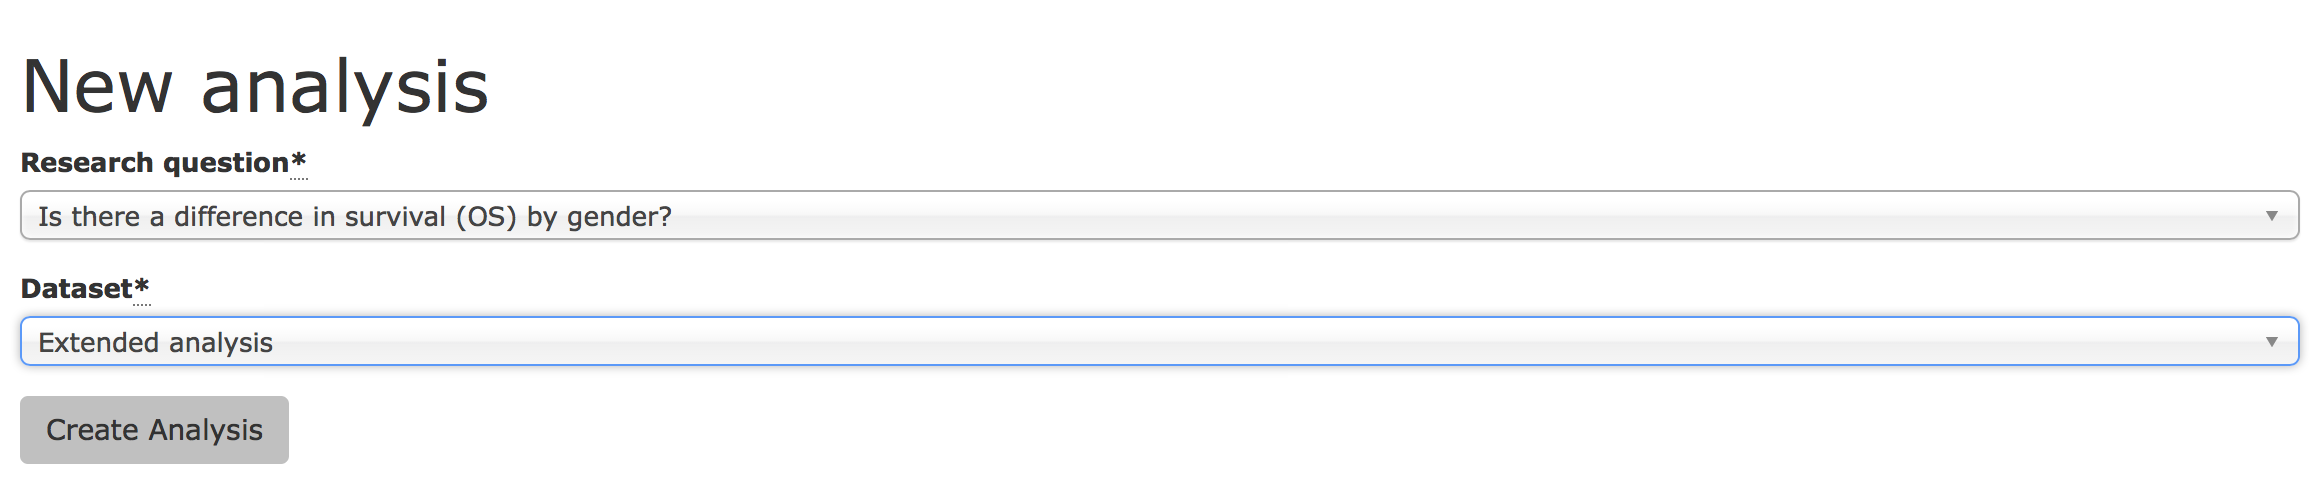
\includegraphics[width=\textwidth]{figures/ui_analysis_0}
	\caption{Creating a new analysis, step 1: Selection of a data set and research question. }
	\label{fig:analysis:1}
\end{figure}

In this particular case, all entered models for the given research question are possible. If one \texttt{TestAssumption} for one of those models would not hold and this model would have further \texttt{Query(Test)Assumptions}, these will not be presented to the end-user, as this model is already not possible anymore. If multiple models require the same answers to one \texttt{QueryAssumption} (e.g. for our example all three models depend on assumption \texttt{A1}) the clinician will only be asked to answer this question once. 

\begin{figure}[h]
	\centering
	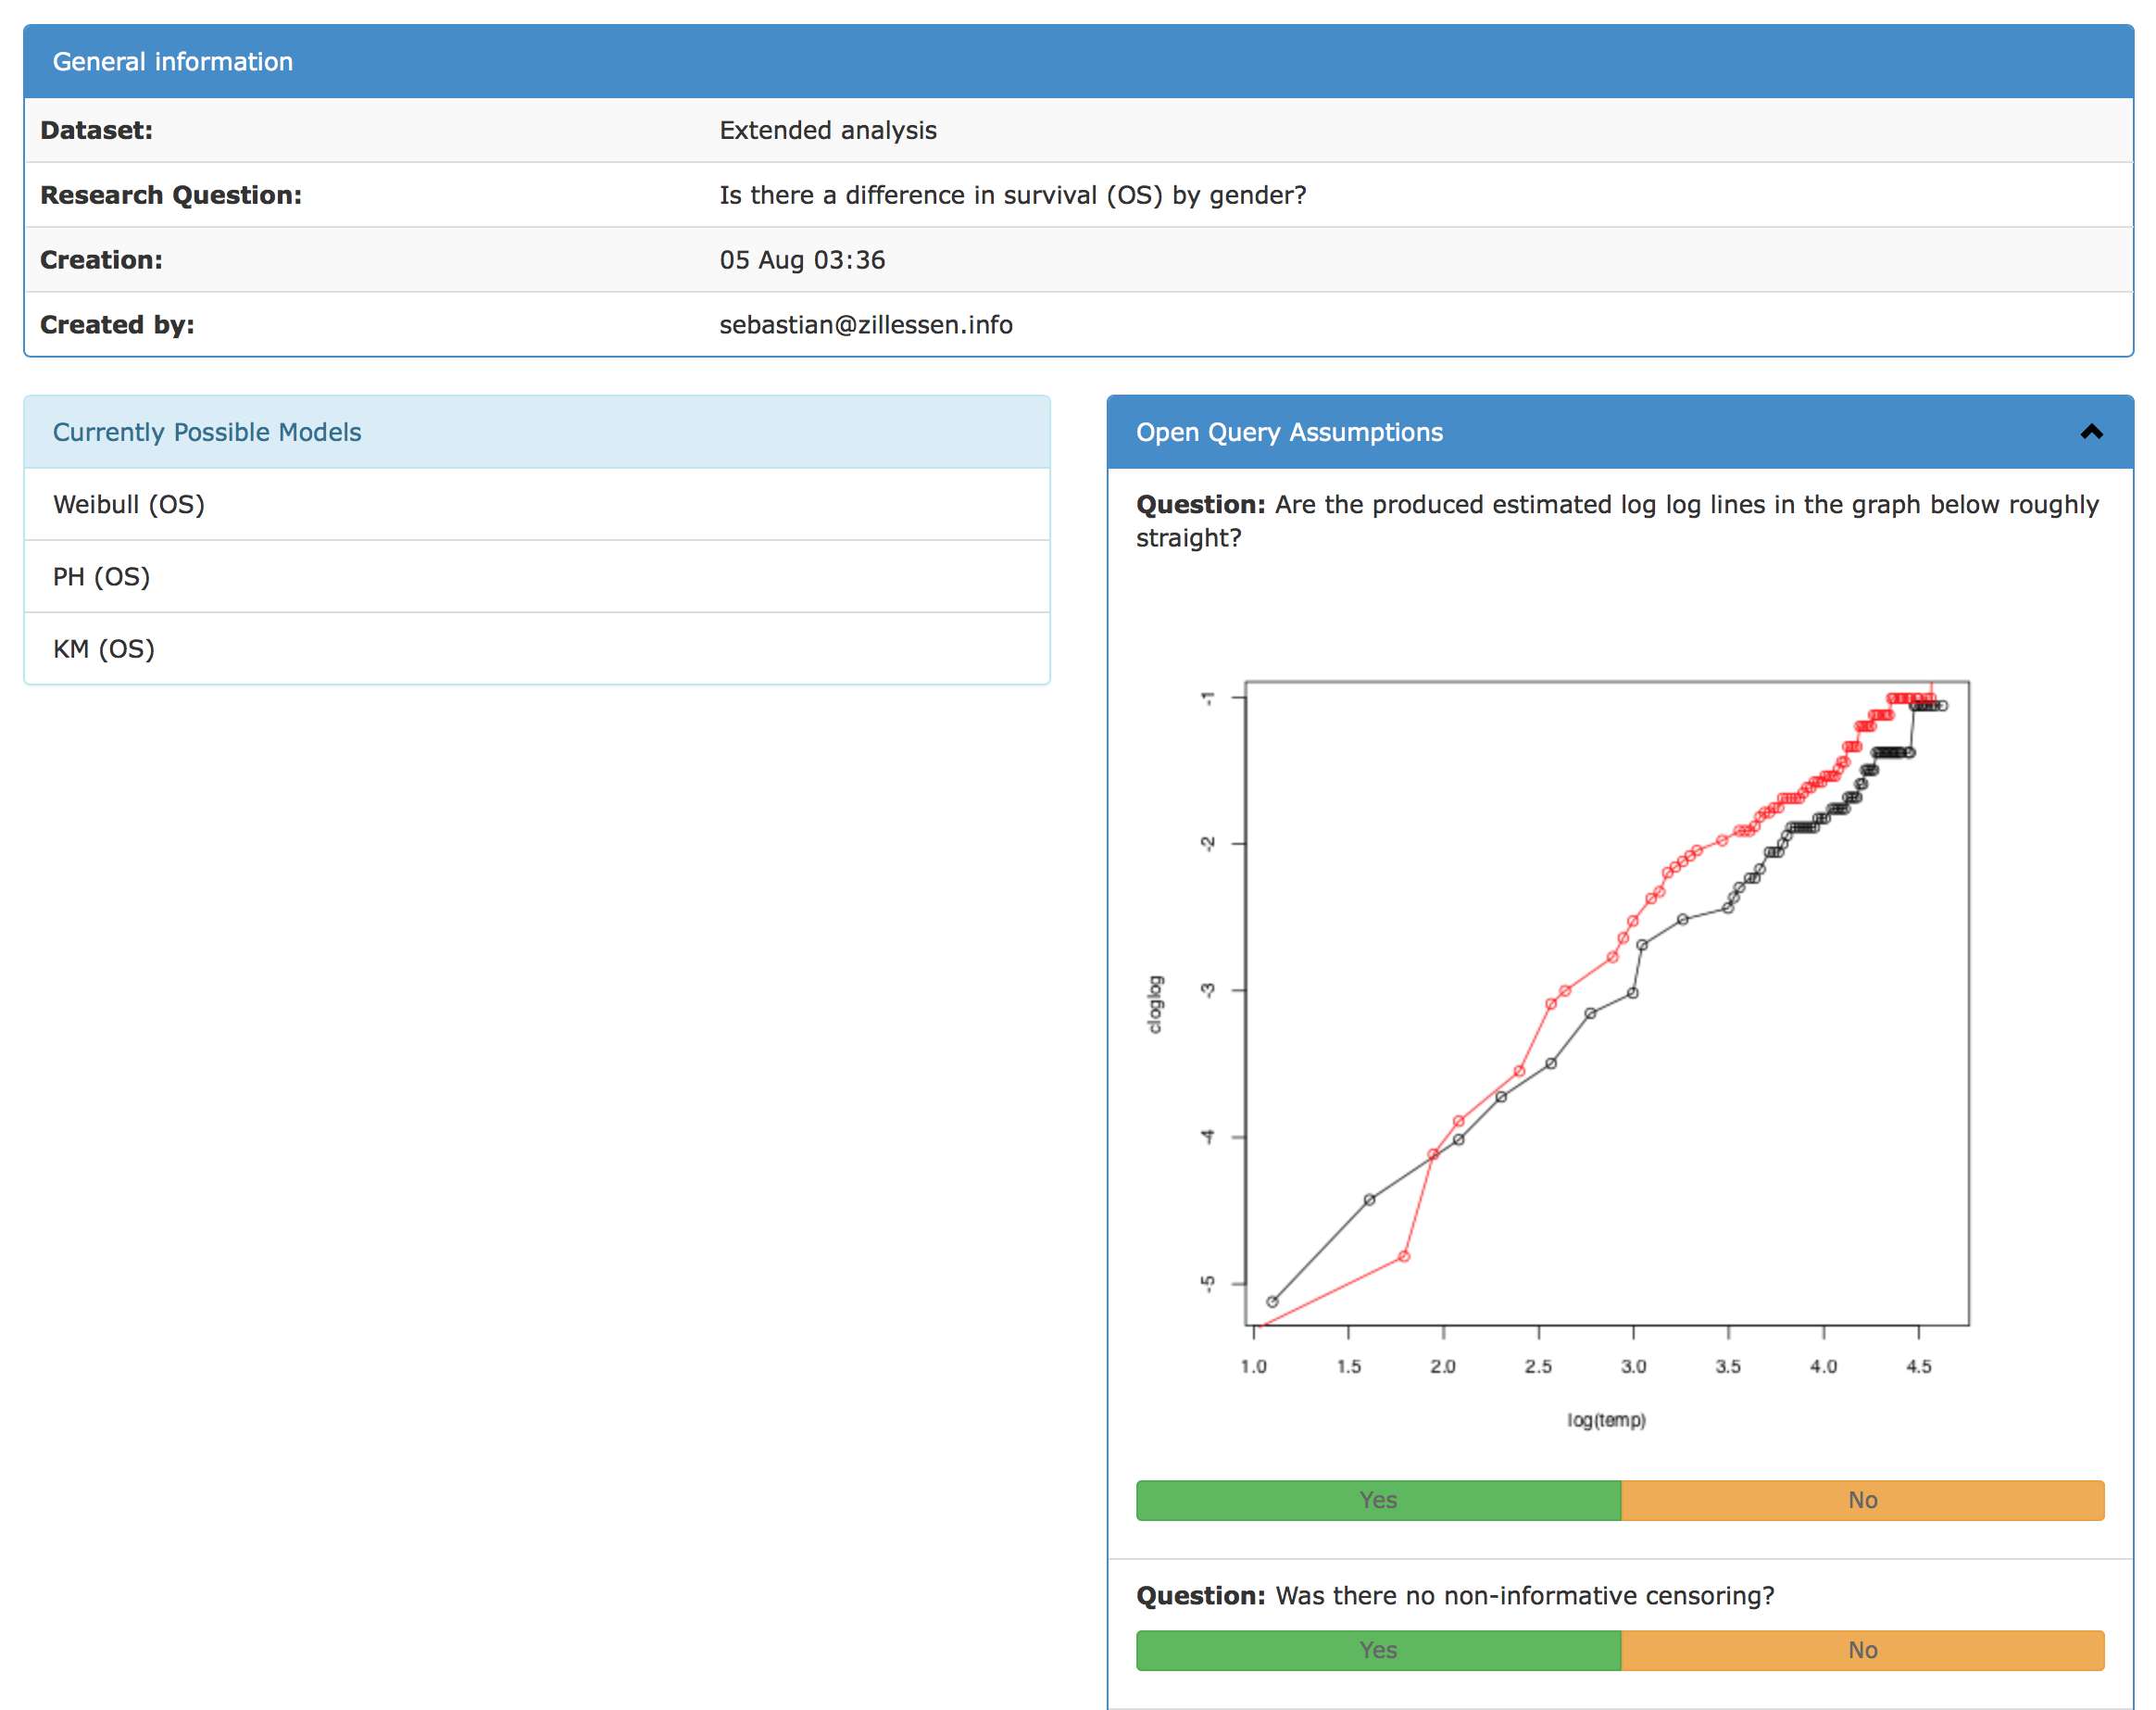
\includegraphics[width=\textwidth]{figures/ui_analysis_1}
	\caption{Creating a new analysis, step 2: Clinician has to answer \texttt{QueryTest-} and \texttt{QueryAssumptions} to perform the analysis. \texttt{TestAssumptions} have already been evaluated.}
	\label{fig:analysis:2}
\end{figure}


As soon as the clinician answers one of the \texttt{QueryAssumptions} the analysis will be updated according to this answer and if some of the \texttt{QueryAssumptions} that are already visible to the user get obsolet by this answer, they will be removed from the open- and moved to the ignored-list (right lower part of \autoref{fig:analysis:3_no}). 
As the clinician answered \texttt{A1} with \textit{No}, the analysis results in no possible models, so no preferences are employed and the analysis is finished.

\begin{figure}[t]
	\centering
	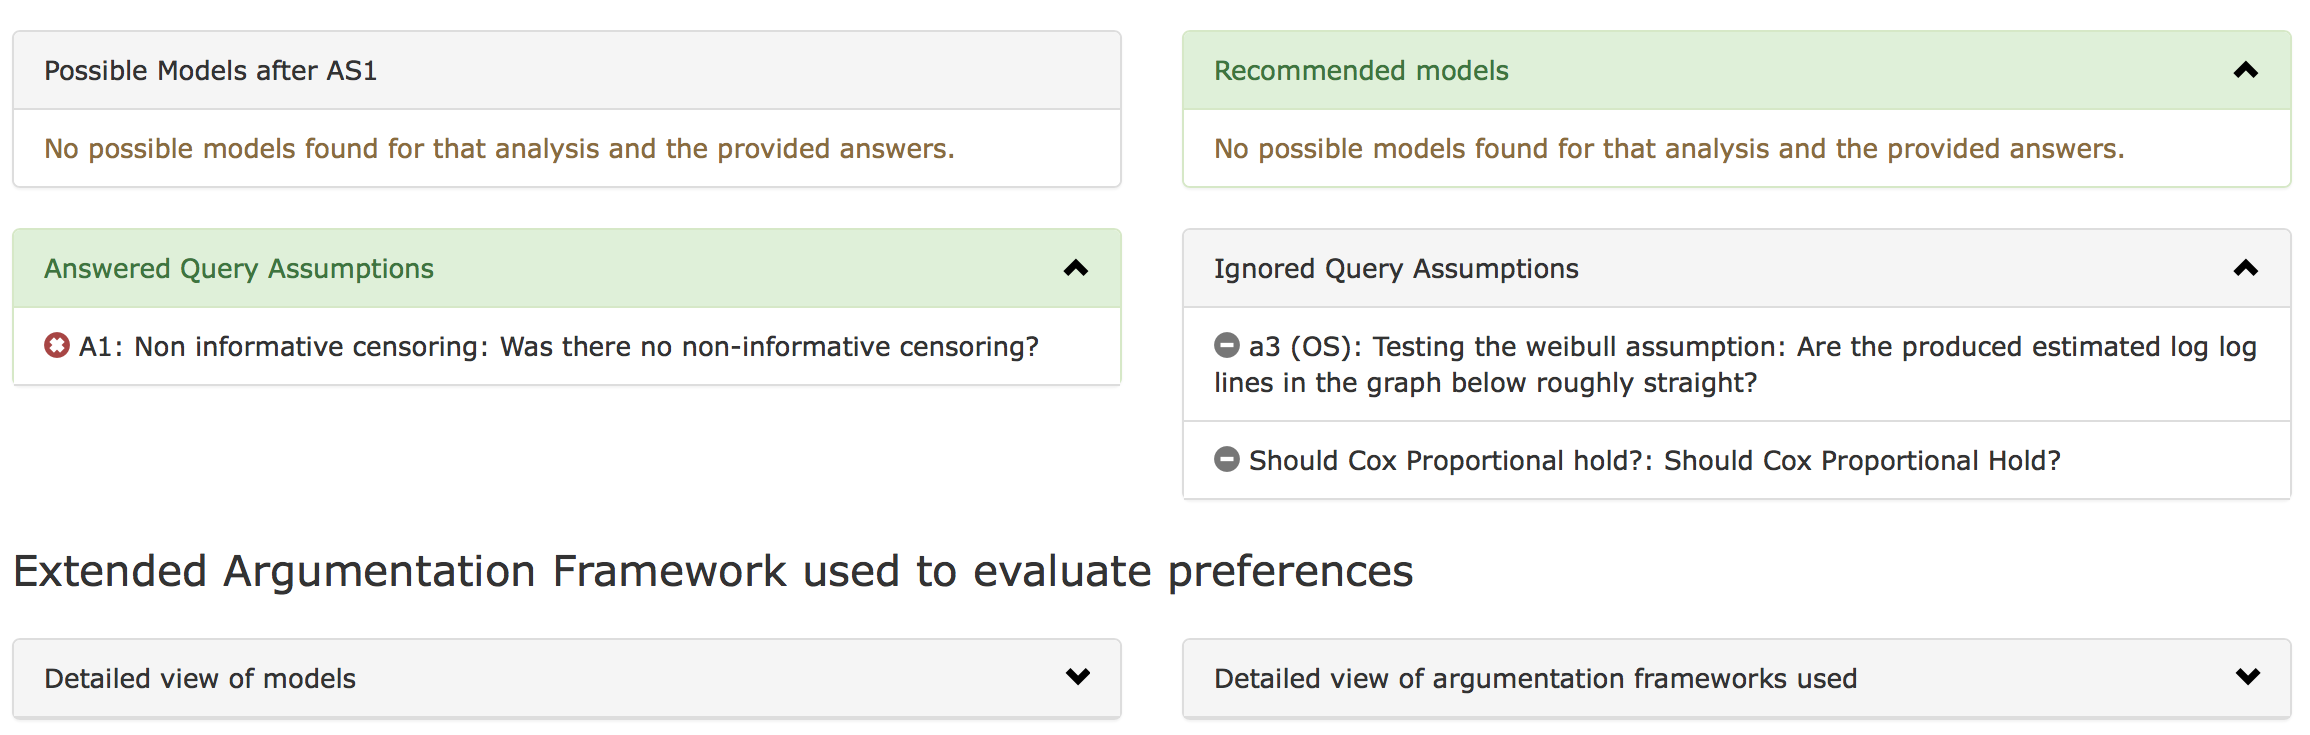
\includegraphics[width=\textwidth]{figures/ui_analysis_2_no}
	\caption{Creating a new analysis, step 3: After answering one question (e.g. "A1: Has no non-informative censoring been in place?" with \textit{No}), the possible models are updated and outdated \texttt{QueryAssumptions} are moved from the list of queries to the list of \textit{Ignored Query Assumptions}.}
	\label{fig:analysis:3_no}
\end{figure}

However, if all \texttt{QueryAssumptions} have been answered positively all three models remain possible. The system will now initiate the \gls{EAF} for this particular analysis as described in \autoref{sub:statistical_model_selection}. The evaluation of this \gls{EAF} is performed in the same order: First, the \texttt{TestAssumptions} are evaluated. Second, if no final solution of the \gls{EAF} could be found, the \texttt{Query(Test)Assumptions} required for the first preference are evaluated. This process is then repeated with the remaining preferences and their \glspl{CD}.

\begin{figure}[t]
	\centering
	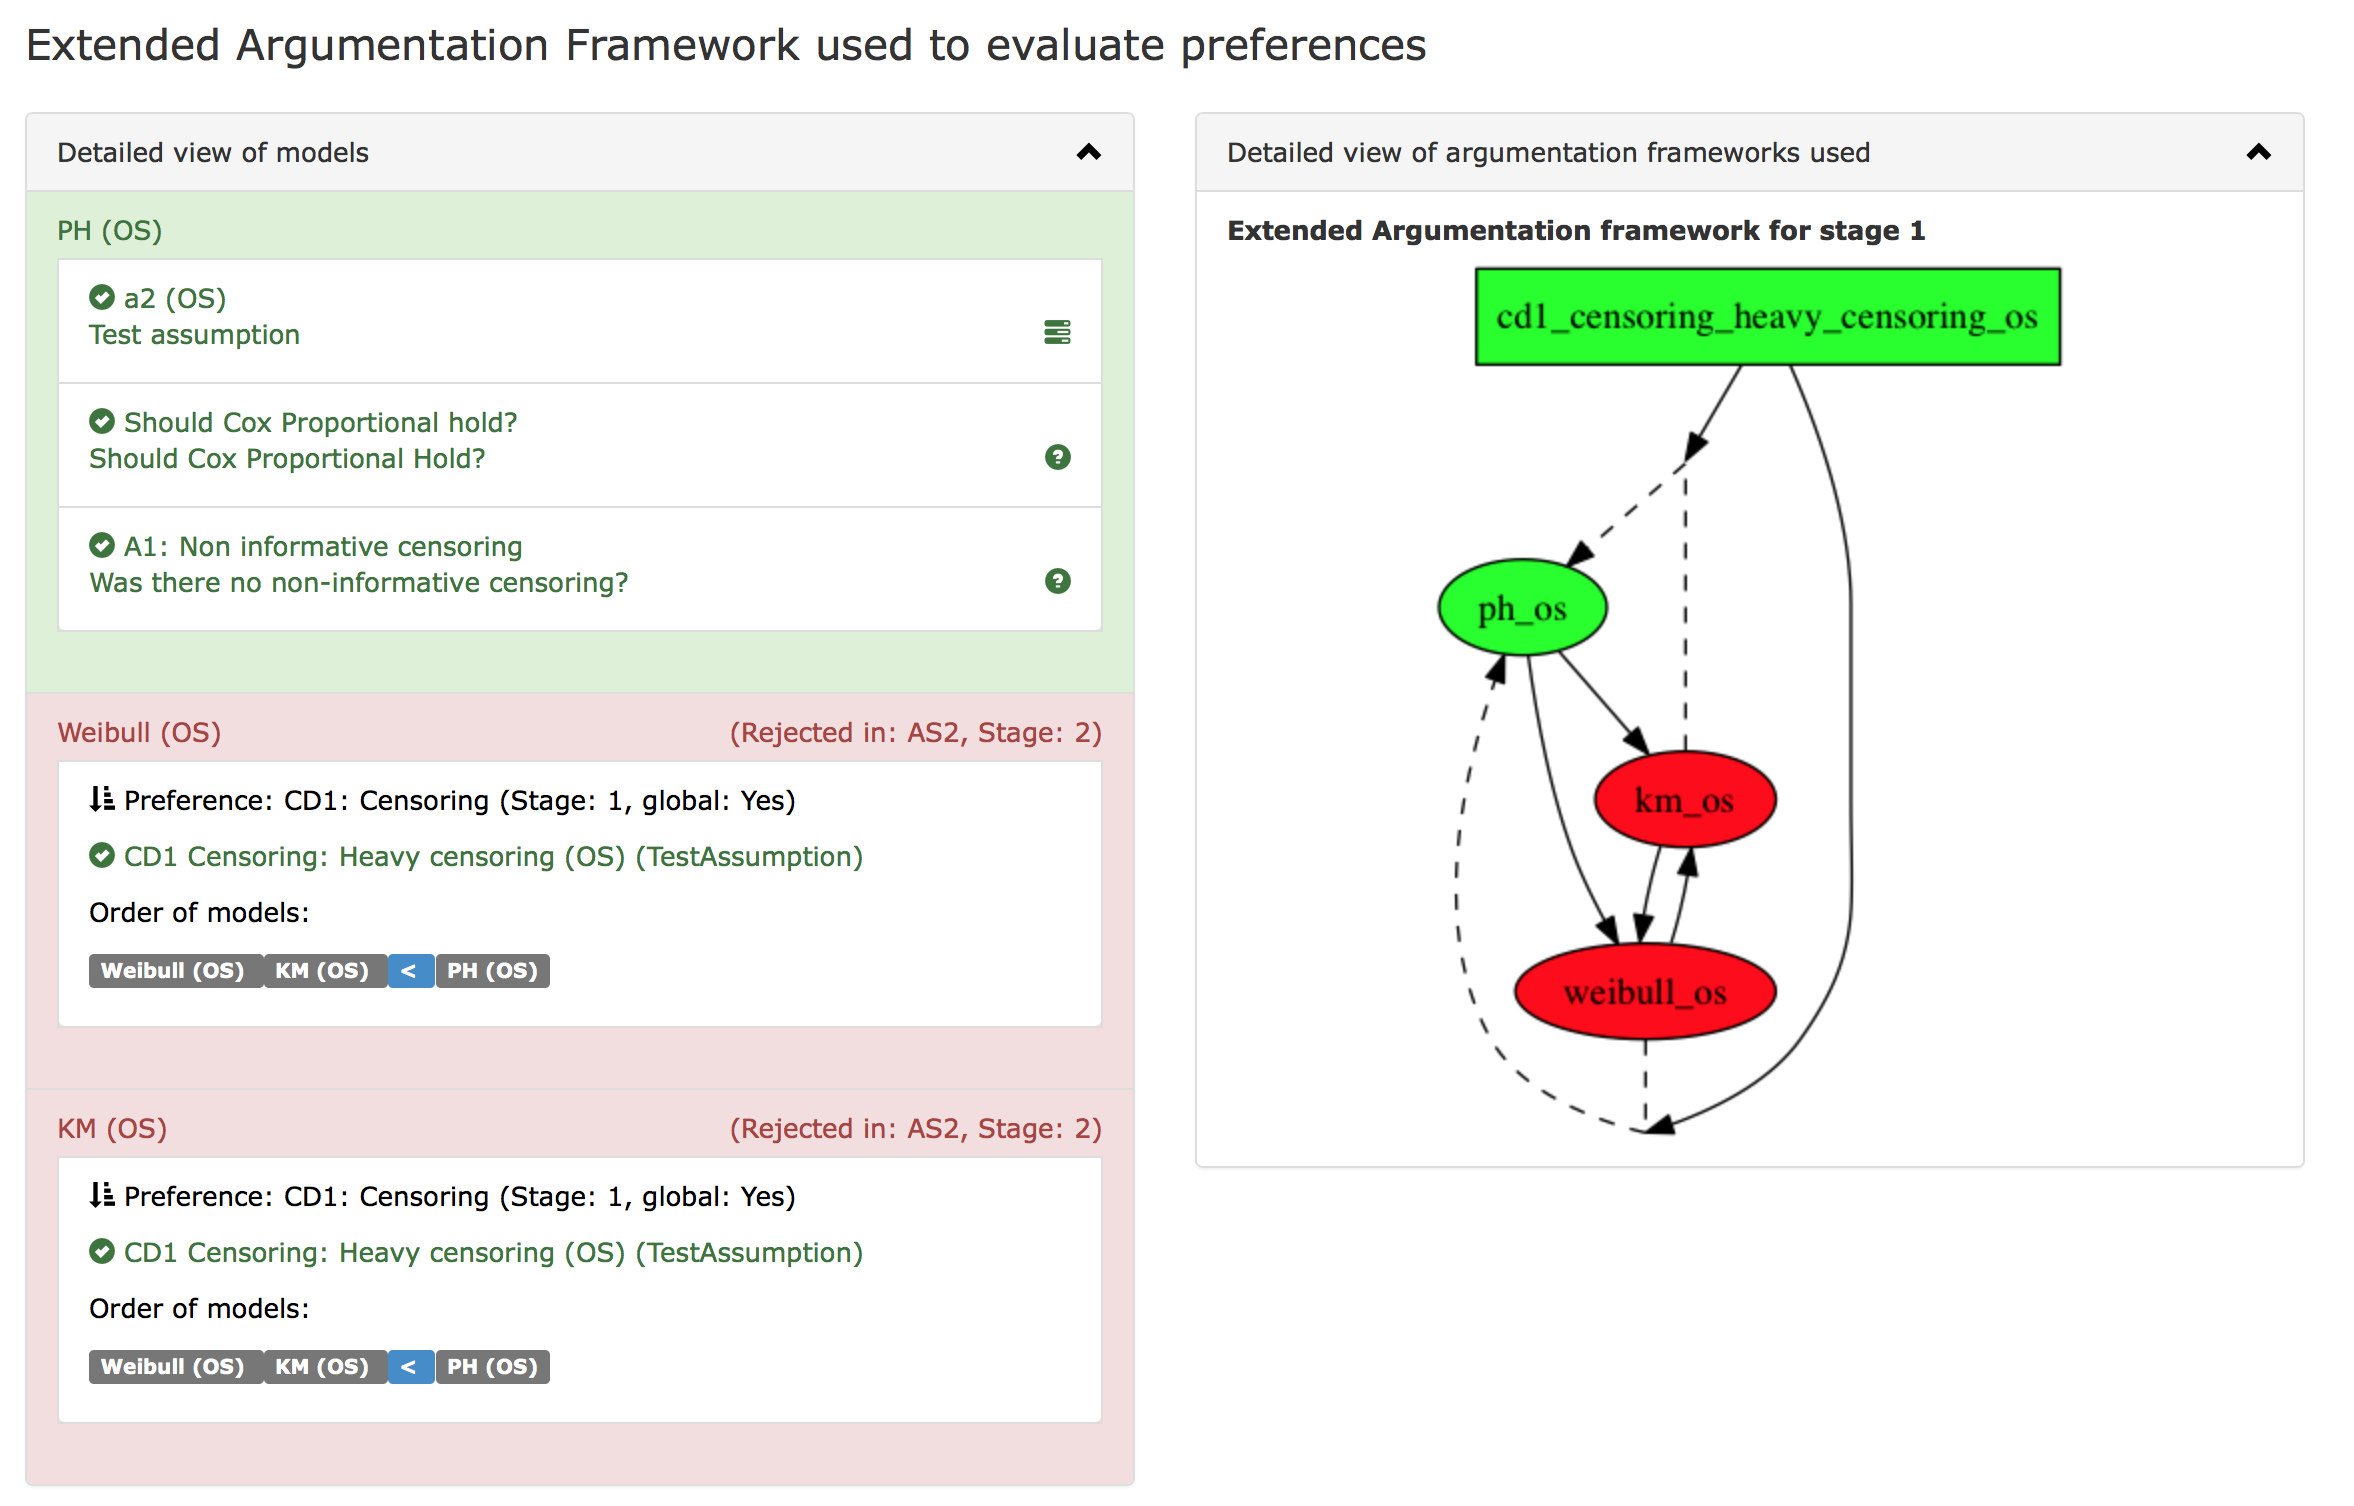
\includegraphics[width=\textwidth]{figures/ui_analysis_eaf}
	\caption{Finished analysis with applied preferences on it: context domain "Censoring" evaluated to \textit{heavy censoring}. }
	\label{fig:analysis:eaf}
\end{figure}


During the evaluation of the preferences per \gls{CD} \textit{Kaplan-Meier} and \textit{Weibull} models are wiped-out as "\textit{Censoring}" has the performance measurement \textbf{heavy}. The generated \gls{EAF} on the right side of \autoref{fig:analysis:eaf} shows the reason why only \textit{Cox-Proportional hazard} remains as the last preferred model.


During the whole process the \gls{UI} provides an interactive way of communication and as it updates its content instantly, the user gets direct feedback on his interaction. In addition, the user is not required to answer all questions in a row, the analysis will still be stored in the system and can be continued at any time. 

\subsection{Observation and Feedback}
\sloppy

The analyses on the provided datasets (as described in \autoref{app:dataset}) are executed rather fast on even larger datasets ($400 \times 15$), as the actual data analysis is done in  \gls{R} scripts that have been used in statistical environments for many years and proofed to be efficient. The results for these scripts are pre-calculated in background processes as soon as the datasets are available. The actual analyses of the different research questions can therefore be performed rather quickly and will be stored for future reference in the database.

The final version of the developed application has been as well tested and evaluated by Isabel Sassoon, scientific assistant of this thesis. As a statistician with a practical knowledge in data mining and consulting clinicians, she could deliver the following feedback on the application (personal communication, August 2016):

In general the developed app fulfils the original defined requirements. In some aspects it provides even more functionality, such as the implementation of contextual factors and argumentation graphs. The overall layout is the same for the expert and the novice user with some of the advanced options being not available for the novice user profile.

Research question can be private or shared, which supports clinicians that are analysing the same data to compare and discuss the best approaches. However, this functionality could be extended in the future to provide the ability to publish research questions to groups of collaborators.


\subsection{Outlooks}
\label{sub:outlooks}

The developed application should be considered as a functional proof of concept and could be extended and improved in various ways. In the following subsection a short list of outlooks is provided (partly based on the Feedback of Isabel Sassoon, personal communication, August 2016).

For a prospective trial roll out to clinicians a pre-population of the application with data (including  all the relevant research questions, models, assumptions and preferences) would be required, as this will provide deeper feedback on the app from an end user perspective.

In addition to this roll out, a trial with statisticians would provide feedback on the underlying mechanisms of the process. This would as well give the chance to verify the system as a statistician could assess whether the recommended models the system reports are the same as he would recommend. 

The results of both above described roll outs could provide a comprehensive analysis of the app and the used methodology. The comparison against a range of criteria could then help to shape any future development plans.

Moreover, an output functionality which covers the steps taken from the research question selected, to the data used, the assumptions tested and the results of the assumptions testing as a summary document could provide better explanation of the process and could be used to develop a statistical analysis plan document (SAP).

Furthermore, as a very demanding client customisation of the layout and the phrasing of texts might be desired to reflect individual workflows in a more efficient way. This could be done during the client specific analysis and be part of a detailed design document.


Especially the process of adding new assumptions and models to research questions can be further improved. For now assumptions rely heavily on the underlying structure of the dataset. To perform two analysis regarding the research questions \textit{"Is there a difference between the survival time for a treatment group in accordance with their {\tiny $\begin{cases} age\\weight \end{cases}$} "} we would need to add the related test assumptions twice into the system. 

This is due to the fact, that the column names in the original datasets should not be changed without documentation as this would conflict the properties of data-provenance \cite{provenance}. As the only changing aspect between the two research questions are the column names \texttt{age} and \texttt{weight}, it would be simpler to map a column name of the data set to a specific column that is required by an assumption which would reduce the number of required assumptions in the system by preventing duplication. For an analysis, the clinician would then have to chose which columns of the dataset should be mapped to which data attribute required by the underlying assumptions. This feature would add high benefits regarding flexibility into the already existing application.

